
\chapter{Physical Reservoir Computing} \label{chapter:lit-prc}

\section{Reservoir Computing} \label{section:rc}
% Where does RC come from?
Reservoir computing (\acrshort{rc}) is a machine learning method proposed in the early 2000s as an alternative to training recurrent neural networks (\acrshort{rnn}) \citep{jaeger_echo_2002}. 
Training weights in recurrent networks requires computationally expensive and highly linear training algorithms such as backpropagation-through-time (\acrshort{bptt}). 
Moreover, \acrshort{bptt} often suffers from numerical instability and often yields suboptimal solutions \citep{bengio_learning_1994}.

In the \acrshort{rc} framework, the untrained \acrshort{rnn} (called the reservoir) is interpreted as a black box dynamical system.
Input signals are transformed by the nonlinear activations of the neurons and are integrated with the past state of the reservoir through recurrent connections \citep{jaeger_harnessing_2004}.
As a result, the reservoir displays both nonlinear behavior and memory capacity.
We can then exploit these properties to solve a variety of regression tasks.


% What does an RC model look like?
\mbox{Figure \ref{fig:rc_diagram}} shows a diagram of a general \acrshort{rc} model using an \acrshort{rnn} as the reservoir.
To accomplish regression tasks, an \acrshort{rc} model consists of two parts: the nonlinear reservoir that transforms environmental inputs and a linear readout function that observes the reservoir to perform a given task. 
The linear readout function observes the state of the reservoir and applies a linear regression model to determine the final output. 
When there is no feedback from the readout function back to the reservoir, it is possible to train multiple readouts that perform different tasks based on the same reservoir dynamics.

\begin{figure}[t]
	\centering
    \includesvg[width=0.65\textwidth]{img/rnn-illustration.svg}
    \vspace{0.35cm}
    % \includegraphics[width=0.5\textwidth]{example-image}
	\caption[A reservoir computing model with a RNN as the reservoir, commonly referred to as an echo state network (ESN).]
	        {A reservoir computing model with a RNN as the reservoir, commonly referred to as an echo state network (ESN).
    	 	 Figure reproduced from \citet{pieters_reservoir_2022} with permission from the author.}
	\label{fig:rc_diagram}
\end{figure}


% What makes RC work?
The key to understanding reservoir computing is that all non-linearity and memory required to solve a given task are already present in the reservoir dynamics. 
The readout function then learns to distill the information present in the observed reservoir state to solve a given task. 
In this way, \acrshort{rc} is similar to the kernel method from classical machine learning, where the reservoir acts as a nonlinear expansion and temporal convolution of the input signals \citep{hermans_recurrent_2012}. 
However, kernel techniques do not account for time explicitly, whereas reservoir computing inherently occurs in the time domain. 
This strong connection to the time domain makes \acrshort{rc} particularly useful for solving tasks with time series data and real-time applications.


% RC is data-efficient and easier to train.
In its original form, the neurons inside the reservoir are randomly connected and are generally not trained. 
However, there is literature that proposes task-independent tuning schemes that improve the stability of the reservoir \citep{lukosevicius_reservoir_2009, norton_preparing_2006, tanaka_effect_2020}.
Reservoir computing models are notably more data-efficient and easier to train because there is no need to train the recurrent part of the network using complex and data-hungry algorithms such as \acrshort{bptt}.


% Concrete frameworks for implementing reservoir computing.
The literature has proposed several implementations of reservoirs.
The echo state network (\acrshort{esn}), as proposed by \citet{jaeger_echo_2002}, is a purely mathematical implementation where neuron activations are determined as a nonlinear function of the weighted sum of incoming connections. 
\acrshort{esn}s operate in discrete time only and are ideal for software implementations.
Subsection \ref{subsection:esn} gives a detailed mathematical description of the echo state network.
Independently, \citet{maass_real-time_2002} proposed the liquid state machine (\acrshort{lsm}), an idea that originated from computational neuroscience.
In this model, the recurrent network is formed by spiking neurons that can operate in both discrete and continuous time.
The neurons receive spike trains (discrete events in time) as input and generate an output sequence of spikes accordingly.
A third approach proposed by \citet{steil_backpropagation-decorrelation_2004} is called Backpropagation-Decorrelation (\acrshort{bpdc}). 
It is a learning algorithm for online training of the readout weights.


\subsection{Echo State Network} \label{subsection:esn}


% introduction
The Echo State Network (ESN) is a mathematical framework that implements the core concepts of reservoir computing \citep{jaeger_tutorial_2002}. 
In this framework, the reservoir is a discrete-time RNN using a sigmoidal nonlinearity (such as the tanh function). 
The activation weights of the reservoir are initialized randomly and remain fixed. 
The linear readout function takes the reservoir state as input and is fit to the desired target signal.

The reservoir state in time step $t$ is calculated from the input signal $\mathbf{u}$ using the following update rules \citep{lukosevicius_reservoir_2012},


\begin{align}
    \tilde{\mathbf{x}}[t] &= \tanh \left( \mathbf{W}^{\text{in}}[1;\mathbf{u}[t]] + \mathbf{W} \mathbf{x}[t-1] \right) \label{esn:update1} \\
    \mathbf{x}[t] &= (1-\alpha) \mathbf{x}[t-1] + \alpha \tilde{\mathbf{x}}[t] \label{esn:update2}
\end{align}


where $\mathbf{x}$ signifies the reservoir neurons' activations, $\mathbf{\tilde{x}}$ the activation update, and $\alpha$ a scalar leaking rate. The readout function $\mathbf{y}$ is fulfilled by a simple linear regression of the reservoir state and an optional direct feed-in of the input signal.

\begin{equation}
\mathbf{y}[t] = \mathbf{W}^{\text{out}}\left[1; \mathbf{u}[t];\mathbf{x}[t] \right] \label{esn:readout}
\end{equation}


The weights $\mathbf{W}^{\text{out}}$ of the readout function can be trained using a variety of learning methods. A common offline approach for fitting the function output to a target signal is ridge regression \citep{lukosevicius_reservoir_2012}:

\begin{equation}
    \mathbf{W}^{\text{out}} = \mathbf{Y}_{\text{target}}\mathbf{X}^{T} \left(\mathbf{X} \mathbf{X}^{T} + \lambda^{2} \mathbf{I} \right)^{-1} \label{esn:training}
\end{equation}

where $\lambda$ is a regularization parameter that prevents overfitting.
For $\lambda$ = 0, the model attempts to find weights that fit the training data exactly.
The results is a high training accuracy, but low accuracy on unseen data.
Large model weights are penalized for $\lambda$ > 0, resulting in smaller weights and a more generalized model.
However, if $\lambda$ is too large, the model parameters shrink too much, and the model loses expressiveness.
The optimal value for $\lambda$ should be selected using validation data separate from training and test data.
Other regression techniques are also possible.
For example, \citet{burms_reward-modulated_2015} have demonstrated online training of the readout function using reward-modulated Hebbian plasticity rules.


\subsection{Applications} \label{subsection:rc_applications}


% Introduction to application domains.
Reservoir computing has enjoyed success in a multitude of research domains because of its simple computational model, the potential for real-time processing, and broad applicability to problems in the physical world \citep{tanaka_recent_2019}. 
Early applications of RC include time series prediction tasks such as stock price forecasting and weather forecasting \citep{nakajima_physical_2020}. 
Table \ref{table:rc-subjects} shows a comprehensive summary of the domains to which RC has been applied as compiled by \citet{tanaka_recent_2019}.
Similarly, \mbox{Table \ref{table:rc-applications-benchmarks}} gives a selection of works that demonstrate the application of reservoir computing. 


\begin{table}[!ht]
    \raggedleft
    \caption[Examples of subjects in RC applications.]{Examples of subjects in RC applications. This table originally appeared in \citet{tanaka_recent_2019} and has been reused under the CC BY 4.0 license.}
    % \def\arraystretch{1.4}%  1 is the default, change whatever you need
    \begin{tabular}{p{0.25\linewidth}  p{0.7\linewidth}}
    \toprule
        \textbf{Category} & \textbf{Examples} \\ \midrule
        Biomedical & EEG, fMRI, ECG, EMG, heart rates, biomarkers, BMI, eye movement, mammogram, lung images. \\ 
        \arrayrulecolor{black!10!white}
        \midrule
        Visual & Images, videos. \\ 
        \midrule
        Audio & Speech, sounds, music, bird calls. \\ 
        \midrule
        Machinery & Vehicles, robots, sensors, motors, compressors,  controllers, actuators. \\ 
        \midrule
        Engineering & Power plants, power lines, renewable energy, engines, fuel cells, batteries, gas flows, diesel oil, coal mines, hydraulic excavators, steam generators, roller mills, footbridges, air conditioners. \\ 
        \midrule
        Communication & Radio waves, telephone calls, Internet traffic. \\ 
        \midrule
        Environmental & Wind power and speed, ozone concentration, PM2.5, wastewater, rainfall, seismicity. \\ 
        \midrule
        Security & Cryptography. \\ 
        \midrule
        Financial & Stock price, stock index, exchange rate. \\ 
        \midrule
        Social & Language, grammar, syntax, smart phone. \\ 
    \arrayrulecolor{black}
    \bottomrule
    \end{tabular}
    \label{table:rc-subjects}
\end{table}



% TODO: make this table prettier (2022-02-17)
% TODO: add references in this table to bibliography (2022-02-17)
\begin{table}[!ht]
    \raggedleft
    \caption[Applications and related benchmark tasks of RC.]{
        Applications and related benchmark tasks of RC. This table originally appeared in \citet{tanaka_recent_2019} and has been reused under the CC BY 4.0 license.
    }
    % \def\arraystretch{1.4}%  1 is the default, change whatever you need
    \begin{tabular}{p{0.25\linewidth}  p{0.7\linewidth}}
    \toprule
        \textbf{Applications} & \textbf{Benchmark tasks} \\ 
        \midrule
        Pattern classification & Spoken digit recognition (Verstraeten, Schrauwen, Stroobandt and Van Campenhout, 2005), 
        Waveform classification (Paquot et al., 2012), 
        Human action recognition (Soh \& Demiris, 2012),
        Handwritten digit image recognition (Jalalvand, Van Wallendael, \& Van de Walle, 2015) \\
        \arrayrulecolor{black!10!white}
        \midrule
        Time series forecasting & Chaotic time series prediction (Jaeger, 2001),
        NARMA time series prediction (Jaeger, 2003) \\
        \midrule
        Pattern generation & Sine-wave generation (Jaeger, 2002), 
        Limit cycle generation (Hauser, Ijspeert, Füchslin, \& Maass, 2012) \\
        \midrule
        Adaptive filtering and control & Channel equalization (Jaeger \& Haas, 2004) \\
        \midrule
        System approximation & Temporal XOR task (Bertschinger \&; Natschläger, 2004), 
        Temporal parity task (Bertschinger \&; Natschläger, 2004) \\
        \midrule
        Short-term memory & Memory capacity (Jaeger, 2002) \\
    \arrayrulecolor{black}
    \bottomrule
    \end{tabular}
    \label{table:rc-applications-benchmarks}
\end{table}

% Tables \ref{table:rc-subjects} and \ref{table:rc-applications-benchmarks} give an overview of subjects to which RC has been applied and references to applications and benchmarks respectively.
% In robotics, RC is deployed as a low-power real-time integrator of sensor data and motor controller  \citep{nakajima_information_2015, burms_reward-modulated_2015}.



% \ref{table:rc-subjects}

% One of the earliest demonstrations of reservoir computing is the Liquid State Machine (2002)\citep{maass_real-time_2002}.

% Since its inception, reservoir computing has been successfully applied in several domains. % though today it has mostly been succeeded by Deep Learning techniques \cite{citation needed}.

% - Example of LSM \cite{maass_real-time_2002}

% - Examples of applications are \cite{lukosevicius_reservoir_2012, nakajima_physical_2020}. see also Tanaka 2019 section 2.2 table 1 and table 2 \cite{tanaka_recent_2019}.

% - Also the source of more theoretical research in mathematics and chaos, see \cite{hermans_recurrent_2012, gauthier_next_2021}

  

\section{Physical Reservoir Computing} \label{section:prc}

% What is physical reservoir computing?
The RC model easily extends to the physical world by interpreting physical systems that exhibit nonlinear dynamics and memory effects as a reservoir substrate  \citep{nakajima_physical_2020}. 
In other words, this Physical Reservoir Computing (PRC) framework aims to exploit dynamics found in the natural world to perform computational tasks. 
% How is RC transferred to the real world?
\mbox{Figure \ref{fig:prc_examples}} shows a mapping of the RNN-based RC architecture to two physical applications from the literature and the plant RC case discussed in this thesis.
In the physical systems (\mbox{Figures \ref{fig:prc_examples}}b, c, and d), it is impossible to observe the complete state of the reservoir as in the RNN-based reservoir. 
Instead, the reservoir state is inferred from sensor data observing the dynamical system in real-time \citep{burms_reward-modulated_2015, nakajima_information_2015}.

\begin{figure}[t]
	\centering
    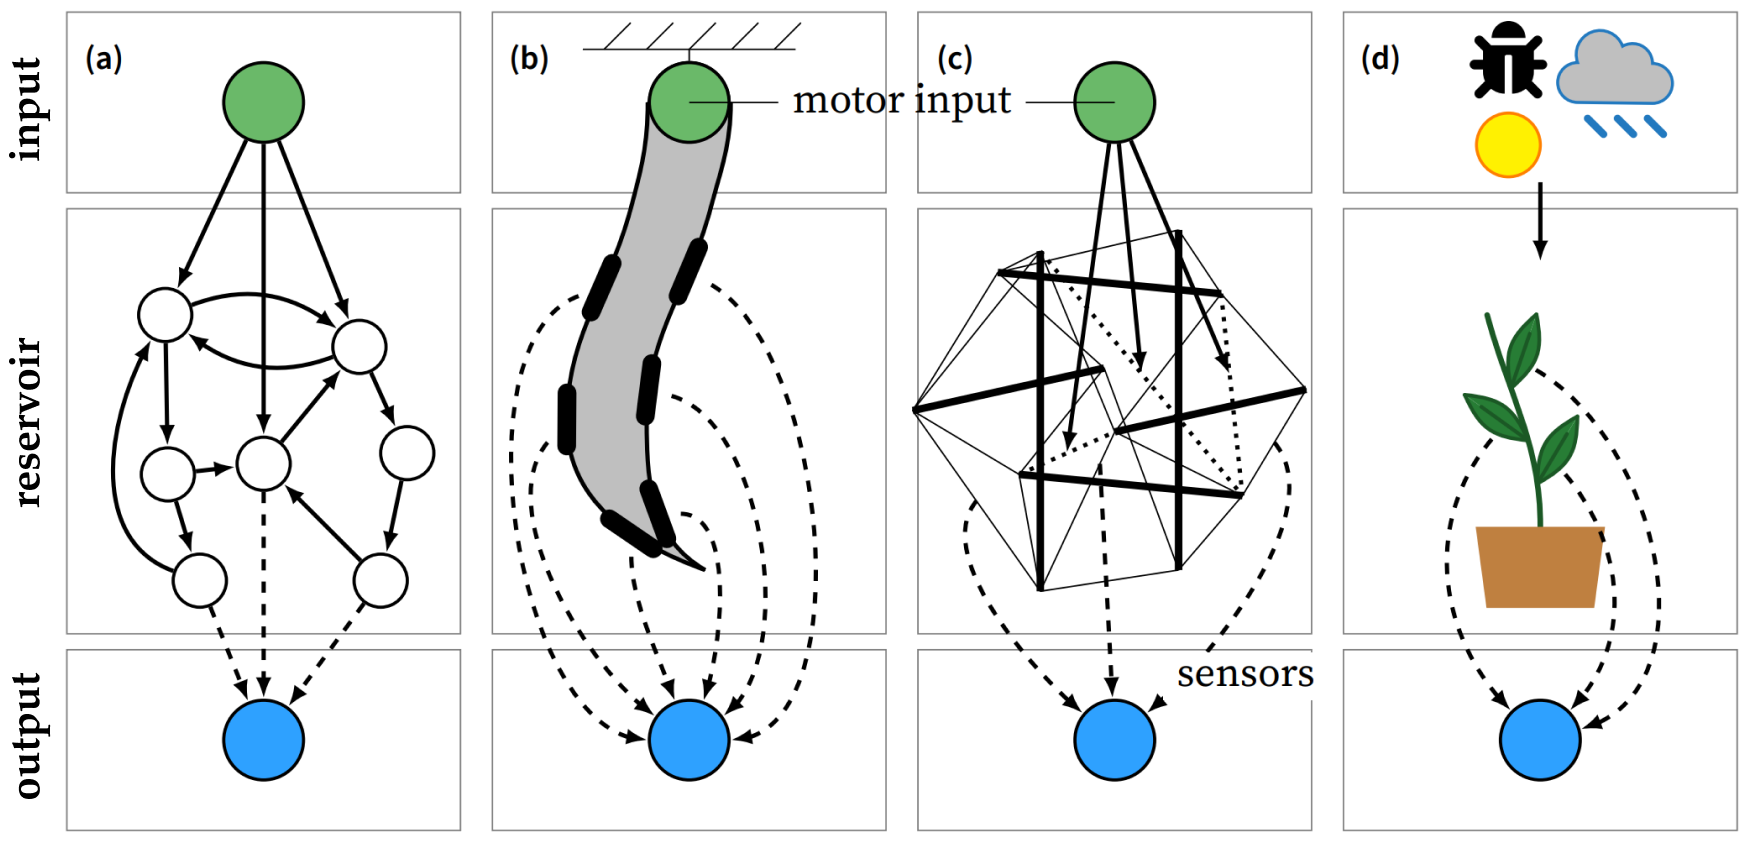
\includegraphics[width=0.9\textwidth]{img/prc-illustration.png}
    % \vspace{0.5cm}
    % \includegraphics[width=0.5\textwidth]{example-image}
	\caption[Illustration of different reservoir computing implementations, both theoretical and physical versions.]
	        {Illustration of different reservoir computing implementations, both theoretical and physical versions. 
	        Each of the subfigures depicts a different type of implementation: 
	            (a) RNN-based version; 
	            (b) soft body built of silicone \citep{nakajima_information_2015}; 
	            (c) compliant robot made of a tensegrity structure \citep{caluwaerts_locomotion_2013}; 
	            and (d) plant as reservoir.
    	 	Figure and caption reused from \citet{pieters_reservoir_2022} with permission from the author.}
	\label{fig:prc_examples}
\end{figure}

% What applications have been made with PRC?
PRC is a field of interdisciplinary research, implementing reservoirs using a large variety of materials \citep{tanaka_recent_2019}.
Examples of substrates being researched are analog electrical circuits \citep{soriano_minimal_2015, zhao_novel_2016}, FPGAs \citep{antonik_application_2018}, memristive circuits \citep{walter_neuromorphic_2015}, photonic circuits \citep{van_der_sande_advances_2017}, spintronics \citep{torrejon_neuromorphic_2017}, and soft body robotics \citep{caluwaerts_body_2011, caluwaerts_design_2014, nakajima_soft_2013}.
Biological reservoirs are closely investigated as well, with a particular interest in neurobiology \citep{hafizovic_cmos-based_2007, hinaut_real-time_2013} and ecological dynamics \citep{jones_is_2007, didovyk_distributed_2015,ushio_computational_2021}. 
Most recently, \citet{pieters_plants_2021} demonstrated promising results in the use of \textit{in vivo} plants as reservoir substrate.


% What is the goal of PRC research?
A common misconception about PRC research is that the goal is to achieve general-purpose computation with unconventional reservoirs. 
However, the aim is not to outperform silicon computers at carrying out generic calculations. 
Instead, in most cases, the goal is to bypass the need for precise modeling of a physical system by observing how the system responds to inputs rather than attempting to predict how the inputs influence the state of the system \citep{nakajima_physical_2020}.
This method is particularly applicable in real-time control scenarios such as robotics, where real-time integration of sensor data is more feasible than power-hungry physics simulations (see e.g.\ \cite{caluwaerts_design_2014, burms_reward-modulated_2015}), 
or for the prediction of chaotic systems where powerful computers are not able to predict the system better than low-powered reservoir models \citep{gauthier_next_2021}.


\subsection{Generalized Mathematical Model} \label{section:rc-general}

The mathematical model of the Echo State Network (section \ref{subsection:esn}) can be generalized to describe any reservoir computer, physical or otherwise \citep{nakajima_physical_2020}. 
Doing so will be helpful to determine what defines the RC system's computational capacity in the following sections. 
This section establishes a mathematical vocabulary for describing any PRC model in discrete-time notation.

The reservoir update function can be described as a function $f(\cdot, \cdot)$ that maps the previous reservoir state and the current input to a new reservoir state,
 
\begin{equation} \label{prc:update}
    \mathbf{x}[t] = f\left(\mathbf{x}[t-1], \mathbf{u}[t]\right) 
\end{equation}

where $\mathbf{x}$ describes the entire reservoir state at step $t$ and $\mathbf{u}$ represents all external factors that influence the dynamics of the reservoir substrate. 
Assuming the reservoir dynamics result in emergent memory effects, it is possible to reformulate the reservoir state $\mathbf{x}$ as a function of the past inputs it has seen:

\begin{equation} \label{prc:echo_input_function}
    \mathbf{x}[t] = \phi(\mathbf{u}[t], \mathbf{u}[t-1], \mathbf{u}[t-2], \dots)
\end{equation}

This function $\phi$ is called the input echo function and is a key characteristic of each particular reservoir substrate. The target task is defined as any arbitrary function $T$ of the past time steps, thus requiring memory to solve:

\begin{equation} \label{prc:target}
    \mathbf{y}[t] = T(\mathbf{u}[t], \mathbf{u}[t-1], \mathbf{u}[t-2], \dots)
\end{equation}

Finally, the linear readout function $\psi$ is described as a learned approximation of $T$, based on the reservoir state:

\begin{align} 
    \psi(\mathbf{x}[t]) &= \psi \left( \phi(\mathbf{u}[t], \mathbf{u}[t-1], \mathbf{u}[t-2], \dots) \right) \label{prc:readout} \\
    &\approx T(\mathbf{u}[t], \mathbf{u}[t-1], \mathbf{u}[t-2], \dots) = \mathbf{y}[t] \nonumber
\end{align}

It is important to note that the input echo function $\phi$ is surjective for virtually all reservoirs. 
In other words, a unique sequence of inputs does not necessarily result in a sequence of unique reservoir states. 
Not only is this natural, as no reservoir can have infinite memory of past events, Section \ref{section:esp} shows that this summarizing property of $\phi$ is vital to derive any meaningful computation from reservoir computers. 

\section{The Echo State Property} \label{section:esp}

% Need for deterministic computations
Strictly speaking, for a reservoir to possess reproducible computational properties, it must show a deterministic relation between its input sequence and its state \citep{nakajima_physical_2020}. 
Put plainly, applying the same input sequence should reliably produce the same sequence of output states.


% Determinism is too strict for physical systems
This precondition is particularly strict on physical systems because it requires precise control over the initial conditions of the physical reservoir (Equation \ref{prc:update}).
This requirement is virtually unattainable as it is impossible to account for all physical factors of an environment that influence the reservoir before the start of the experiment.
Fortunately, a lesser but sufficient condition exists to perform useful computation with a reservoir.


% The echo state property comes to the rescue
The echo state property (\acrshort{esp}) (also referred to as the fading memory property) defines a less strict precondition under which it is possible to derive computations from a dynamical system.
Informally, the \acrshort{esp} states that a sufficient condition for reservoir computing is for the input echo function $\phi$ (Equation \ref{prc:echo_input_function}) to have fading memory of past inputs \citep{lukosevicius_reservoir_2012}. 
If this assumption is valid, then the trajectories of the reservoir state will converge when subjected to the same input sequence, regardless of the initial conditions.
A side-effect of the echo state property is that it limits the reservoir's memory of past events, thus limiting the available integration window for memory-bound tasks.


% Example in ESN.
Figure \ref{fig:fading_mem_principle} demonstrates the principle using an ESN. It shows the evolution of a single node in the network for two runs. 
At step 0, we initialized the reservoir state with a different random state vector. 
After step 0, we subject the reservoir to the same input sequence for both scenarios.
While the initial trajectory depends on the node's starting value, the neuron synchronizes to the input sequence entirely by step 75. 
The node's evolution no longer depends on the initial value from that point onwards.



% Fading memory can be recognized in many systems
Fading memory can be recognized in physical dynamical systems as well.
Oftentimes it is the result of a dampening force such as electrical resistance or drag.
For example, \citet{nakajima_information_2015} implemented \acrshort{prc} using a silicone octopus arm submerged in water. 
In their particular case, the. fluid resistance of the water tank exerts a dampening effect on the silicone arm, resulting in a fading memory.


% The mathematical reason why this works is still being researched
The understanding behind this property is that the response of many dynamical systems eventually synchronizes to the input signal, suppressing chaotic behavior \citep{nakajima_physical_2020}. 
However, the mathematical understanding of the \acrshort{esp} and its relation to dynamical systems is still a topic of active research (see e.g.\ \cite{yildiz_re-visiting_2012, lu_attractor_2018}).

\begin{figure}
    \centering
    \begin{subfigure}[b]{0.35\linewidth}
        \centering
        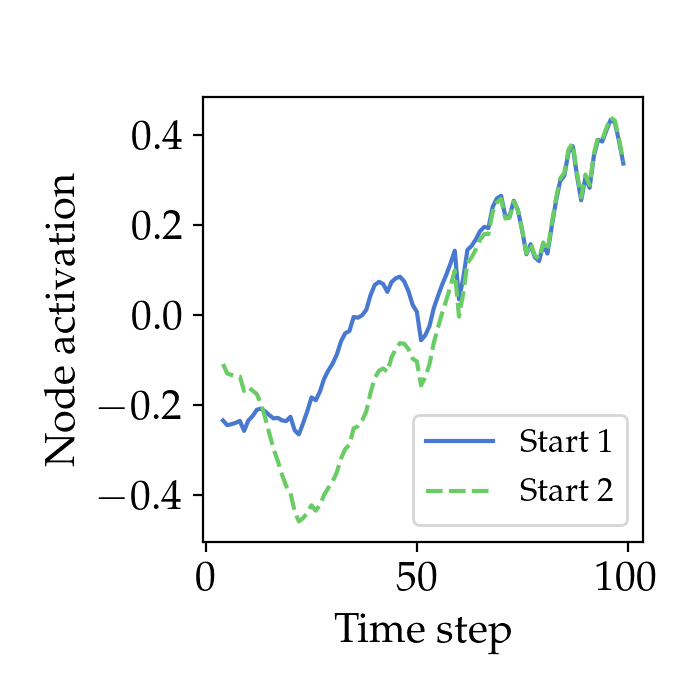
\includegraphics[height=5.7cm,keepaspectratio]{img/explainer_fading_mem.png}
        \caption{ }
        \label{fig:fading_mem_principle}
    \end{subfigure}
    \hfill
    \begin{subfigure}[b]{0.62\linewidth}
        \centering
        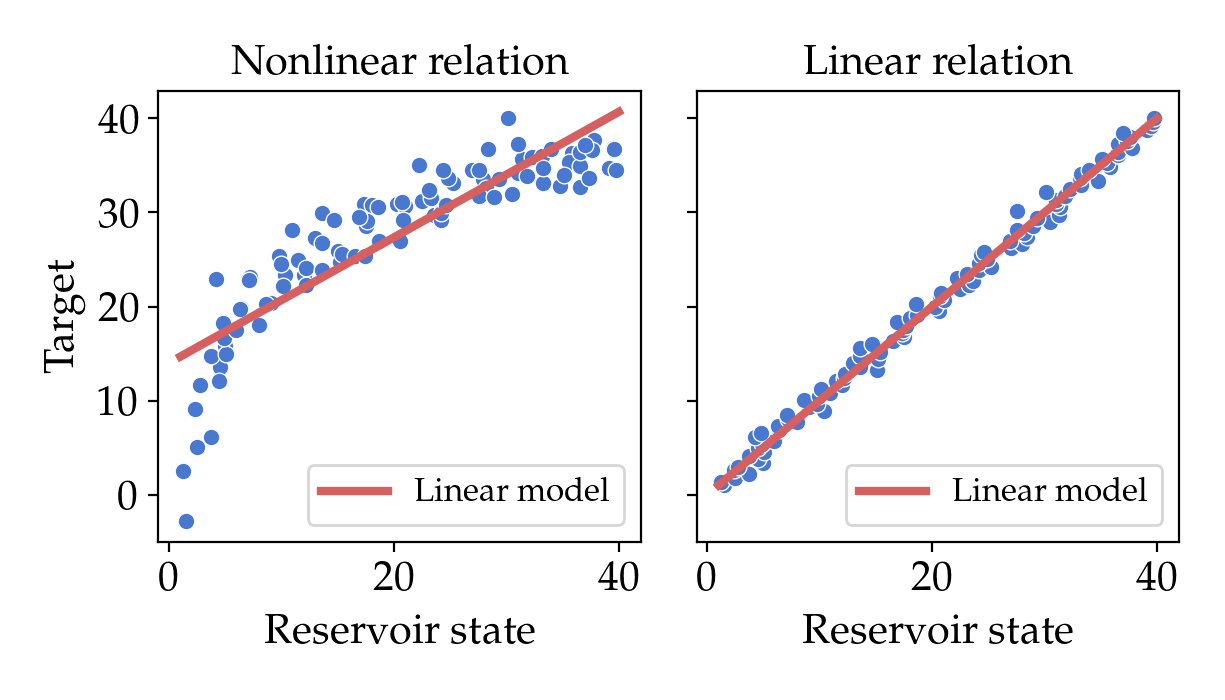
\includegraphics[height=5.7cm,keepaspectratio]{img/explainer_input_sep.png}
        \caption{ }
        \label{fig:input_sep_principle}
    \end{subfigure}
    \caption[Demonstration of the Echo State Property and illustration of linear input separation.]{
        Demonstration of the Echo State Property and illustration of linear input separation.
        (\subref{fig:fading_mem_principle}) Demonstration of the \acrlong{esp} in an ESN with 100 nodes, leak rate 0.16 and spectral radius 1.25. The ESN is subjected to the same input sequence, with two different initial state vectors. The plot shows the activation value of the same node through time.
        (\subref{fig:input_sep_principle}) Example of linear input separation between a target task and the reservoir state. The left plot shows a nonlinear relation (in this case, logarithmic). The right plot shows a linear relation. The red line shows a linear regression model fitted to the data.
    }
    \label{fig:prc_principles}
\end{figure}



\section{Time Scale of Reservoir Dynamics} \label{section:rc-time-scales}

% Reservoirs can have a wide range of time scales
As Section \ref{section:rc} already stated, reservoir computing occurs inherently in the time domain.
That means we must carefully consider the time scale at which the reservoir dynamics occur.
The time scale of reservoir dynamics can vary significantly. 
For example, imagine a physical reservoir implemented as a resistive-capacitive electrical network. 
The time it takes for the network to reach a resting state can be changed by increasing or decreasing the resistance and capacitance of the elements present in the network.
We can tune the dynamics' time scale to range from milliseconds to minutes or hours.


% Effect of time scale on memory capacity
A faster time scale also means the reservoir returns to its resting state faster, decreasing the system's memory capacity. Figure \ref{fig:leak_rate_verstraeten} from \citet{verstraeten_towards_2009} illustrates the effect of time scale on memory capacity.
The plot shows the memory capacity for ESNs with twenty nodes and different leak rates. The smaller the leak rate, the wider but flatter the memory curve becomes.
That means that networks with a lower leak rate show better long-term memory at the cost of precision in memory of more recent inputs.

\begin{figure}[]
	\centering
    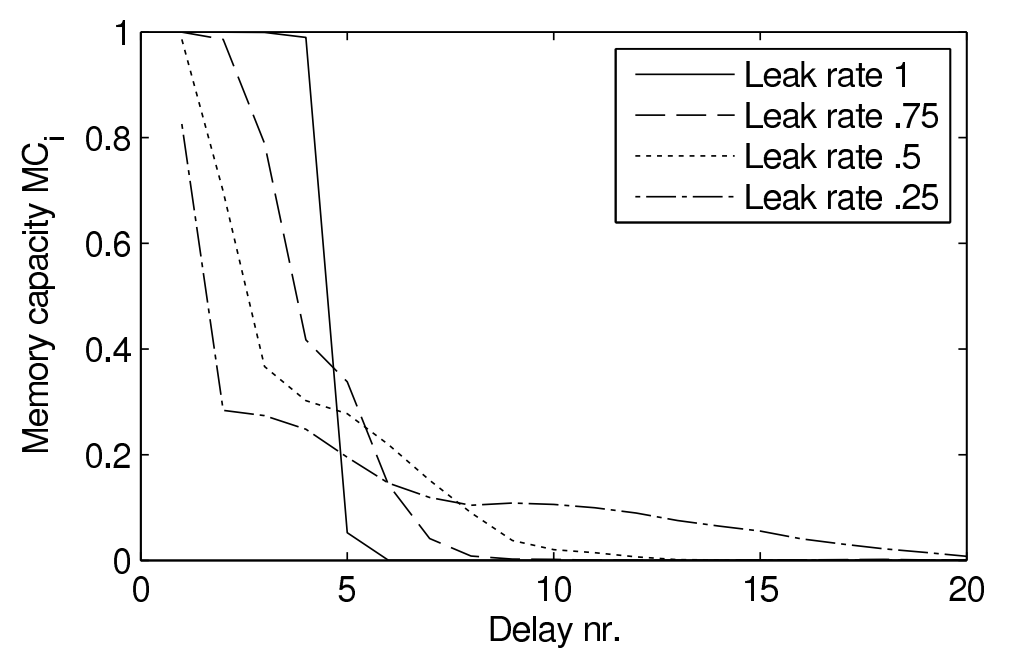
\includegraphics[width=0.55\textwidth]{img/leak_rate_verstraeten.png}
	
	\caption[Memory capacity for \acrshort{esn}s with different leak rates (from \citet{verstraeten_towards_2009}).]{
    		Memory capacity for \acrshort{esn}s with different leak rates (see Subsection \ref{subsection:esn}). Networks with a smaller leak rate show better long-term memory at the cost of decreased accuracy in short-term memory. This figure originally appeared in \citet{verstraeten_towards_2009}.
        }
	\label{fig:leak_rate_verstraeten}
\end{figure}


% This is shown in Figure 3.2. In this plot, the memory curve for a reservoir of 20 tanh nodes
% is shown with dierent leak rates. The plot shows that decreasing leak
% rates cause the memory curve to become flatter and wider. This means
% that the reservoir has worse memory of recent inputs, but better memory of inputs further in the past. Thus, by decreasing the leak rate we
% increase the longer-term memory of the nodes at the expense of precision
% in recalling the more recent inputs.


% Takeaway for reservoir computing
The takeaway here is that the time scale of the reservoir dynamics plays a vital role in its ability to solve a given task. 
A reservoir highly synchronized to its inputs will display faster dynamics and thus a shorter but greater precision integration window for solving tasks.
Conversely, a reservoir with higher memory capacity will typically exhibit slower dynamics and thus a longer integration window, at the expense of short-term precision.


\subsection{Sampling of a Continuous-Time Reservoir}

% What is the problem when sampling a continuous-time signal?
While the dynamics of a physical reservoir operate in continuous time, most applications implement the readout model digitally using a conventional computer and sensors that discretely sample the input signals and reservoir state.
According to the Shannon-Nyquist sampling theorem, to sample a continuous signal without losing information we must sample at twice the rate of the largest frequency component present in that signal \citep{shannon_communication_1949}.
Hence, determining the right time scale at which the desired reservoir dynamics occur plays a prominent role in PRC system design. 
Undersampling critical signals in the reservoir will result in information loss by introducing aliasing in the sampled signal. 
In conclusion, effectively sampling the reservoir state presents an additional optimization problem when implementing RC with physical reservoirs.


% What are the problems with undersampling or oversampling?
% Sampling at a higher frequency than the reservoir dynamics that can solve the desired task adds high-frequency noise to the signal. 
% The presence of this additive noise can degrade the performance of the linear readout function. 


% - TODO: Maybe here I can add a figure that is a toy demonstration of under and oversampling in an RC system?

 

\section{Evaluating Reservoir Performance} \label{section:reservoir-eval}

% Introduction to the different properties of a reservoir to be benchmarked.
Before attempting to solve a specific computational task, it is important to 
map out what the physical reservoir can do by benchmarking its computational properties.
To have computational capacity, a reservoir should show input separability and fading memory \citep{nakajima_information_2015}.
Evaluating these properties is in fact a way of characterizing the echo response function of the system as described in Section \ref{section:rc-general}.
% To determine the computational capacity of a reservoir, we must evaluate it on three key fronts: (i) input separability; (ii) fading memory property; (iii) memory capacity \citep{nakajima_information_2015, nakajima_physical_2020}.

% Q: add (iv) stationarity?

\subsection{Input Separability}

% What is input separability
The readout function is a strictly linear model. 
To solve nonlinear tasks, the reservoir must transform its inputs such that the task becomes a linear function of the reservoir state.
In other words, there must be a linear relation between the reservoir's observable state and the target task.
Figure \ref{fig:input_sep_principle} shows an example of linear input separation in a reservoir.

However, the nonlinear transformation applied by a finite reservoir cannot solve any arbitrary task.
In addition, the presence of notable recurrent effects in the reservoir may degrade precision in recalling recent inputs (Section \ref{section:rc-time-scales} explores this phenomenon further).
When the input transformation applied by the reservoir results in an observable state from which a readout function can compute the desired task efficiently, we speak of good input separability.
Good input separability is a function of both nonlinearity and memory, and the optimal mix of both properties varies depending on the task.


% How to measure input separability
One way to evaluate the input separation of a reservoir relative to a given task is to train a reservoir readout and a control readout model \citep{ushio_computational_2021}. 
The former fits to the reservoir state, while the latter fits to the environmental signals directly.
If the expanded state of the reservoir contains helpful input separation for the task, the reservoir readout will perform better than the control model.


\subsection{Fading Memory} \label{sec:fading_memory}

% Introduction to fading memory
Section \ref{section:esp} already stated the importance of fading memory in physical reservoirs.
However, this property is difficult to measure directly.
Nonetheless, we will outline two ideas for measuring this property in physical systems.


% Method 1: warmup time
The first method attempts to measure the warmup time of the reservoir. 
The idea is simple: initialize the same reservoir with different starting conditions, then measure the time it takes for the reservoir state to synchronize to the input.
If the physical system displays the fading memory property, then the trajectories of the reservoirs will eventually synchronize, even if initialized with different starting conditions.
Figure \ref{fig:memory_esn_start} demonstrates this method on an \acrshort{esn} with different leak rates. 
In this experiment, An \acrshort{esn} is subjected to identical input series with two different initial reservoir states $\mathbf{x}$.
The rate at which the reservoir syncs to the input signal depends on the time scale of the reservoir dynamics dictated by the leak rate.

% Method 2: signal spike
In the second method, we subject two reservoirs to identical input signals. 
One reservoir will serve as the test subject, while the other acts as a control.
After the two systems have synchronized to the input, we briefly apply an environmental impulse to the test reservoir, after which the original input signal resumes.
We then measure the time for the test reservoir to resynchronize with the control reservoir.
This impulse can look different depending on the type of reservoir. 
For example, we can temporarily remove the reservoir from its environment such that it no longer receives any environmental stimuli.
Another possibility is to apply an unexpected and artificial stimulus for a short time.
Regardless of how we realize the impulse, we must apply it long enough to have a noticeable impact on the trajectory of the reservoir dynamics.
Otherwise, it is impossible to measure the time until the reservoir synchronizes to the regular inputs.
Figure \ref{fig:memory_esn_impulse} demonstrates this method on an \acrshort{esn}.
This time, all input values between time steps 60 and 80 are set to a fixed value of ten times the standard deviation of the input signal.
After step 80, the reservoir gradually returns to its original behavior, at a rate proportional to its leak rate.


% Measuring divergence in trajectories
Both methods rely on measuring the divergence in behavior of a reservoir when subjected to different conditions. 
To quantitatively compare the difference between reservoir states at time $t$, we can use a distance metric such as \acrfull{mse} on its observable state $X$:

\begin{equation} \label{eq:MSE}
    \text{MSE}(t) = \frac{1}{N} \sum_{i=1}^{N} \left( X_i^{(1)}(t) - X_i^{(2)}(t) \right)^{2}
\end{equation}

where $N$ is the size of the reservoir's observable state vector.


% Relation to memory capacity.
Note that in both experiments, the time it takes for the reservoirs to synchronize also informs about its recurrent dynamics and memory capacity.

\begin{figure}
    \centering
    \begin{subfigure}[b]{0.485\linewidth}
        \centering
        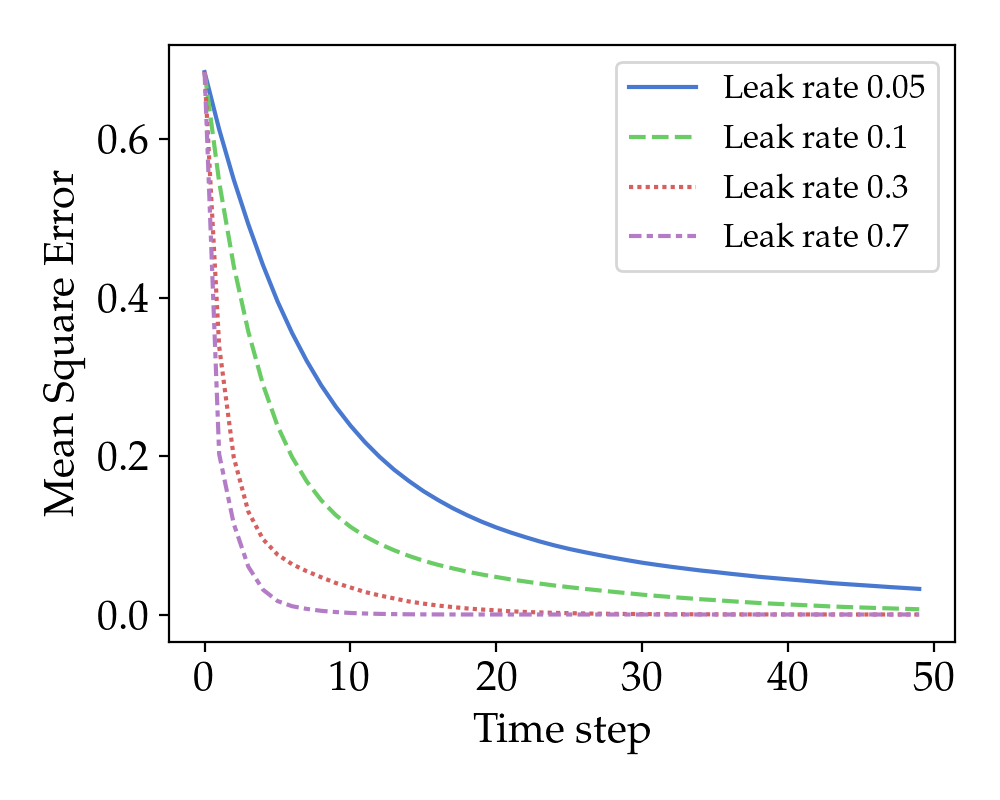
\includegraphics[width=\linewidth,height=\linewidth,keepaspectratio]{img/esn_starting_conditions.png}
        \caption{First method: divergence between reservoirs}
        \label{fig:memory_esn_start}
    \end{subfigure}
    \vskip\baselineskip
    \begin{subfigure}[b]{0.485\linewidth}
        \centering
        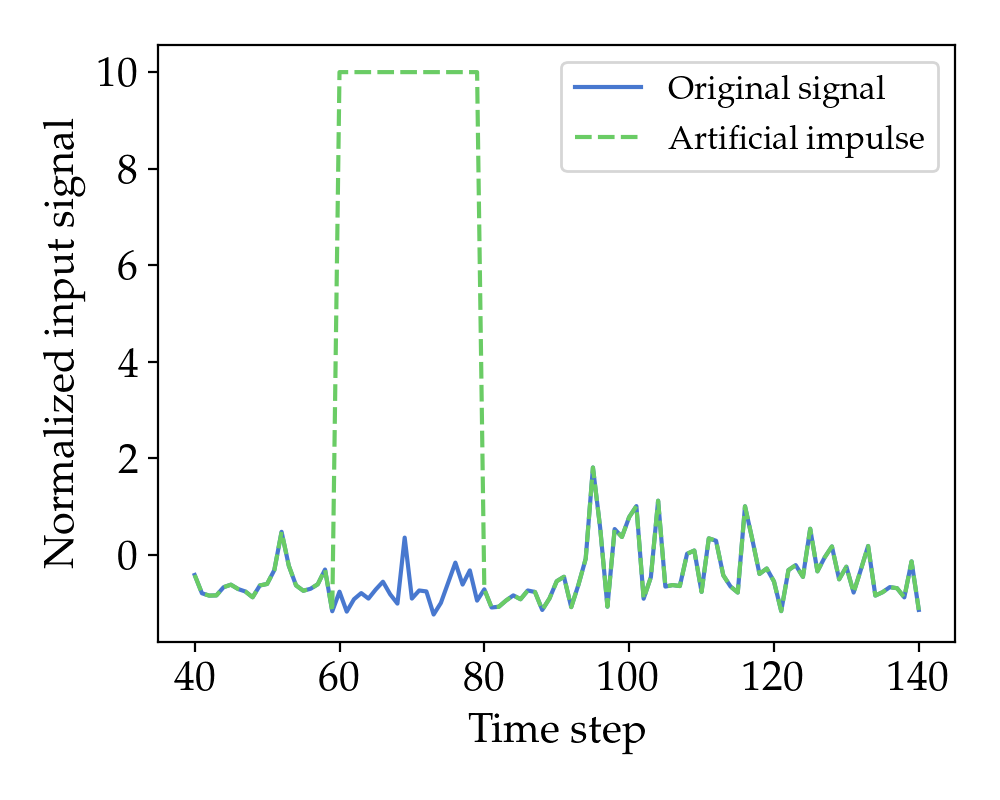
\includegraphics[width=\linewidth,height=\linewidth,keepaspectratio]{img/input_impulse.png}
        \caption{Second method: applying an artificial impulse}
        \label{fig:memory_input_impulse}
    \end{subfigure}
    \hfill
    \begin{subfigure}[b]{0.485\linewidth}
        \centering
        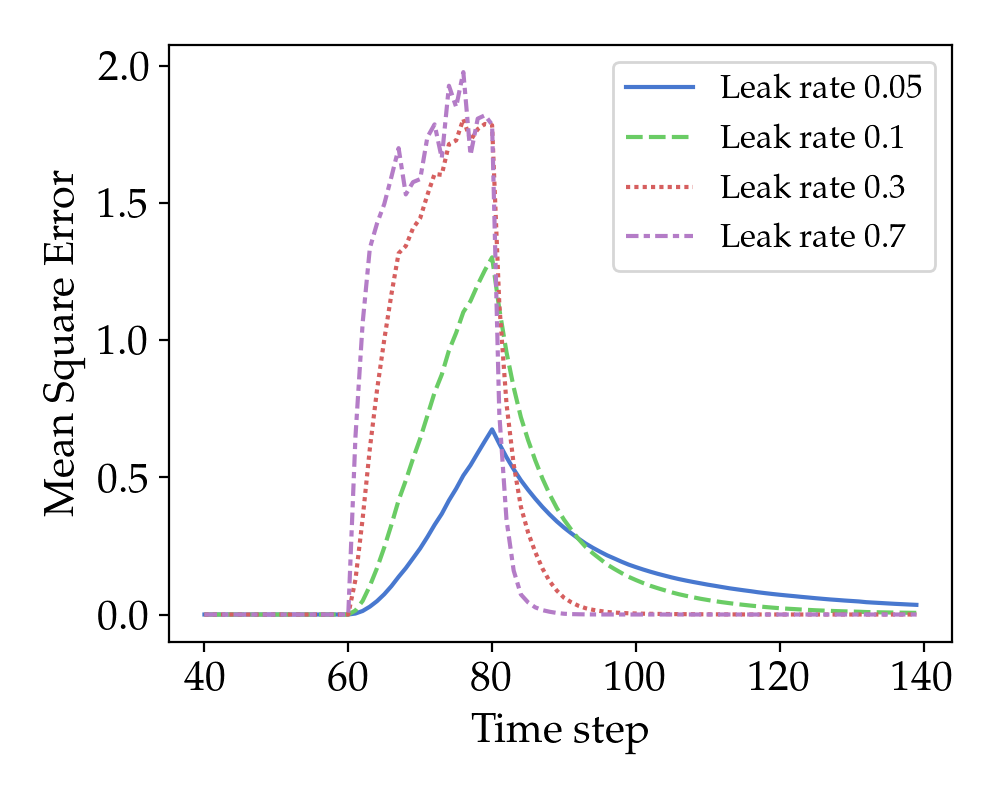
\includegraphics[width=\linewidth,height=\linewidth,keepaspectratio]{img/esn_impulse.png}
        \caption{Second method: divergence between reservoirs}
        \label{fig:memory_esn_impulse}
    \end{subfigure}
    \caption[Two methods for testing the fading memory property of a reservoir, demonstrated using a \acrshort{esn}.]{
            These figures show experimental data from testing the fading memory property of an \acrshort{esn} as described in Subsection \ref{sec:fading_memory}. 
            Both experiments use a reservoir of 100 nodes with randomly initialized weights. 
            For stability, we normalized the weights to have a spectral radius below 1.25 \citep{caluwaerts_design_2014}.
            As input data, we used the California Housing regression dataset \citep{kelley_pace_sparse_1997} which can be found in the sklearn Python package.
            (\subref{fig:memory_esn_start}) The divergence in reservoir state between two runs of the same reservoir with identical inputs and different starting state vectors. 
            The starting states are sampled from a uniform distribution between -1 and 1.
            The disparity between the reservoirs is measured by the MSE between their respective state vectors (Equation \ref{eq:MSE}).
            (\subref{fig:memory_input_impulse}) An artificial impulse with an amplitude of ten times the standard deviation of the original signal is applied between time steps 60 and 80.
            (\subref{fig:memory_esn_impulse}) The divergence in reservoir state between two runs of the same reservoir using identical starting conditions. One run receives an artificial impulse between time step 60 and 80 on all input dimensions, as depicted by Subfigure \subref{fig:memory_input_impulse}.
    }
    \label{fig:fading_memory_experiments}
\end{figure}



\subsection{Computational Benchmarks}

% NARMA
To better compare results between studies of different reservoirs, some standard benchmarks appear in the literature.
The most common \acrshort{rc} benchmark is the nonlinear autoregressive moving average (\acrshort{narma}).
We can tune the nonlinearity and memory of the \acrshort{narma} task With the $n$ parameter.
The \acrshort{narma} system is defined as:

\begin{equation} \label{prc:narma}
    y(t+1) = \alpha y(t) + \beta y(t) \left[ \sum_{i=0}^{n-1} y(t-i) \right] + \gamma x(t-n+1) x(t) + \delta
\end{equation}

where the parameters $\alpha$, $\beta$, $\gamma$, and $\delta$ are set to 0.3, 0.05, 1.5 and 0.1 \citep{nakajima_information_2015}.

For some reservoirs, it is necessary to tune the NARMA system's memory to the correct time scale to get stable results \citep{pieters_reservoir_2022}.
For this the adapted formula can be used:

\begin{equation} \label{prc:narma-timescale-adapted}
    y(t+1) = \alpha y(t) + \beta y(t) \left[ \sum_{i=0}^{n-1} y(t-\tau i) \right] + \gamma x(t-\tau n+1) x(t) + \delta
\end{equation}

where $\tau$ is tuned to the desired time scale of the NARMA system's memory.


% Delay line and polynomial expansion
We can use other simple benchmarks to evaluate the memory and nonlinear properties.
For example, predicting the past inputs of the reservoir for increasing delay tests the memory of the system:

\begin{equation} \label{prc:delay-line-benchmark}
    y(t) = x(t-\tau)
\end{equation}

where greater values of $\tau$ require more memory to solve ($\tau > 0$). 
To test reservoir nonlinearity, a simple exponentiation of the input signal can be used as the prediction target:

\begin{equation} \label{prc:polynomial-benchmark}
    y(t) = (x(t))^{n}
\end{equation}

where $n$ is greater or less than 1.


% Chaotic systems
Finally, to test a reservoir's ability to predict the trajectory of chaotic systems, \citet{ushio_computational_2021} have proposed a test using strange attractors.
In this test, a time series of a Lorenz attractor acts as the input to the reservoir.
The reservoir then has to predict near-future values of this input time series.
The test evaluates how well the reservoir can synchronize with a chaotic system, which is a common application for \acrshort{rc} \citep{tanaka_recent_2019}.


\section{Simulation of Physical Reservoirs} \label{section:prc-simulation}
If the behavior of the $\phi$-function is understood completely, it is possible to create a computer model that simulates the reservoir dynamics \citep{nakajima_physical_2020}. 
Using a simulated reservoir can have various advantages in research. 
(i) It is possible to iterate faster on designing synthetic physical reservoirs, such as FPGAs or photonic circuits, by validating designs in software before constructing the physical reservoir.
(ii) Some reservoirs operate at long time scales \citep{ushio_computational_2021}. Simulation can accelerate the research cycle by running experiments faster than in real-time.
(iii) In simulation, it is possible to operate in a highly controlled environment, which makes it possible to solve a constrained version of a problem first. 
For example, it is possible to dictate identical initial conditions in every experiment run or enforce static reservoir dynamics where the physical counterpart may experience some malleability caused by the environment.

\section{Summary} \label{section:prc-summary}

This chapter showed how physical reservoir computing outsources computation to physical dynamical systems.
This works thanks to the emergent computational qualities present in nonlinear dynamical behavior.
A simple linear readout function is used to transform the reservoir's state into a useful output.
In computer models, we can observe the reservoir state directly.
In physical implementations, we observe the reservoir using sensor data.

To perform useful computations, the reservoir must perform the suitable nonlinear transformations and convolutions to its inputs such that the problem becomes linear.
Another condition for \acrshort{prc} is a fading memory of past inputs; Fading memory is essential to performing deterministic computations.

To test whether a physical material is suitable for reservoir computing, we can design a suite of regression targets to quantify the reservoir's correlation with relevant computational tasks.
In addition, we proposed two types of experiments for testing the fading memory condition: one measures the dependence on initial conditions, and the other measures the stationarity of the reservoir dynamics in time.